\documentclass[a4paper]{article}
\usepackage[utf8]{inputenc}
\usepackage[spanish, es-tabla]{babel}

\usepackage{amsmath}
\usepackage{amsfonts}
\usepackage{amssymb}

\usepackage{float}
\usepackage{graphicx}
\graphicspath{ {./Imagenes/} }

\usepackage{multirow}
\setlength{\doublerulesep}{\arrayrulewidth}

\usepackage{array}
\newcolumntype{C}[1]{>{\centering\let\newline\\\arraybackslash\hspace{0pt}}m{#1}}

\usepackage[american]{circuitikz}

\usepackage{fancyhdr}

\usepackage{units} 

\pagestyle{fancy}
\fancyhf{}
\lhead{22.01 Teoría de Circuitos}
\rhead{Mechoulam, Lambertucci, Rodriguez, Londero}
\rfoot{Página \thepage}



\begin{document}

%%%%%%%%%%%%%%%%%%%%%%%%%%%%%%%%%%%%%%%%%%%%%%%%%%%%%%%%%%%%%%%%%%%%%%%%% 
%								CARATULA								%
%%%%%%%%%%%%%%%%%%%%%%%%%%%%%%%%%%%%%%%%%%%%%%%%%%%%%%%%%%%%%%%%%%%%%%%%% 

\begin{titlepage}
\newcommand{\HRule}{\rule{\linewidth}{0.5mm}}
\center
\mbox{\textsc{\LARGE \bfseries {Instituto Tecnológico de Buenos Aires}}}\\[1.5cm]
\textsc{\Large 22.01 Teoría de Circuitos}\\[0.5cm]


\HRule \\[0.6cm]
{ \Huge \bfseries Trabajo práctico N$^{\circ}$5}\\[0.4cm] 
\HRule \\[1.5cm]


{\large

\emph{Grupo 3}\\
\vspace{3px}

\begin{tabular}{lr} 	
\textsc{Mechoulam}, Alan  &  58438\\
\textsc{Lambertucci}, Guido Enrique  & 58009 \\
\textsc{Rodriguez Turco}, Martín Sebastian  & 56629 \\
\textsc{Londero Bonaparte}, Tomás Guillermo  & 58150 \\
\textsc{Galdeman}, Agustín & 59827\\
\end{tabular}

\vspace{20px}

\emph{Profesores}\\
Jacoby, Daniel Andrés\\
Belaustegui Goitia, Carlos\\
Iribarren, Rodrigo Iñaki\\
\vspace{3px}
%\textsc{} \\	

\vspace{100px}

\begin{tabular}{ll}

Presentado: & */*/19\\

\end{tabular}

}

\vfill

\end{titlepage}


%%%%%%%%%%%%%%%%%%%%%%%%%%%%%%%%%%%%%%%%%%%%%%%%%%%%%%%%%%%%%%%%%%%%%%%%% 
%								INFORME									%
%%%%%%%%%%%%%%%%%%%%%%%%%%%%%%%%%%%%%%%%%%%%%%%%%%%%%%%%%%%%%%%%%%%%%%%%%

\section{Introducción}

En el presente informe se estudiaron distintos tipos de filtros con un enfoque analítico teórico, práctico y además computacional. Para facilitar esto último se creó una interfaz gráfica que logra superponer distintas curvas obtenidas mediante cálculos teóricos de transferencias, mediciones con osciloscopio o simulaciones con LTSpice.

\section{Desarrollo}

\subsection{Ejercicio 1: Filtro Twin T Notch}

Se diseñó el filtro Twin T Notch mostrado en la Figura (\ref{fig:filtroinicial}). Este filtro posee una frecuencia de corte de $ 8.1 \ kHz $. Para eso se requerían resistencias de $ 9 \ k\Omega $ y $ 4.5 \ k\Omega $ (se seleccionaron resistencias de $ 6.8 \ k\Omega $ y $ 2.2 \ k\Omega $ para obtener los $ 9 \ k\Omega $ y una de $ 4.7 \ k\Omega $ en vez de $ 4.5 \ k\Omega $, debido a la consideración de los valores comerciales) y capacitores de $ 4.7 \ nF $ y $ 2.2 \ nF $. De aquí en más se considera $ R = 9 \ k\Omega $ y $ C = 2.2 \ nF $.

\begin{figure}[H]
	\centering
	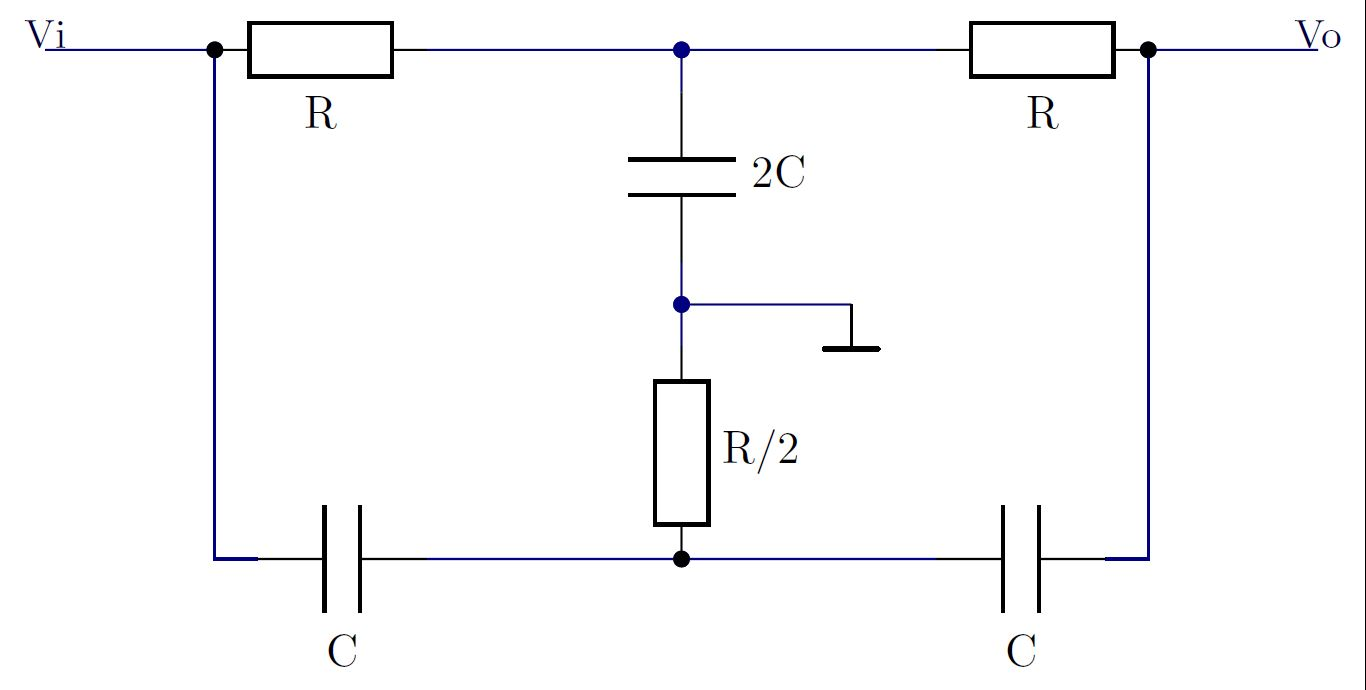
\includegraphics[width=0.6\textwidth ,trim={0 0.1cm  0.1cm 0},clip]{ej1inicial.jpg}
\caption{Filtro Twin T Notch sin simplificar, tomando en consideración las relaciones dadas entre resistores y capacitores.}
	\label{fig:filtroinicial}
\end{figure}

Aplicando el teorema de Kennelly para transformar T a Pi, se obtiene el circuito simplificado de la Figura (\ref{fig:filtrosimplificado}), donde se tiene que
\[Z_1=\frac{1+SCR}{SC}\hspace{1em};\hspace{1em} Z_2=2R(1+SCR) \hspace{1em};\hspace{1em} Z'_2=\frac{2(SCR+1)}{R(SC)^2}\]

\begin{figure}[H]
	\centering
	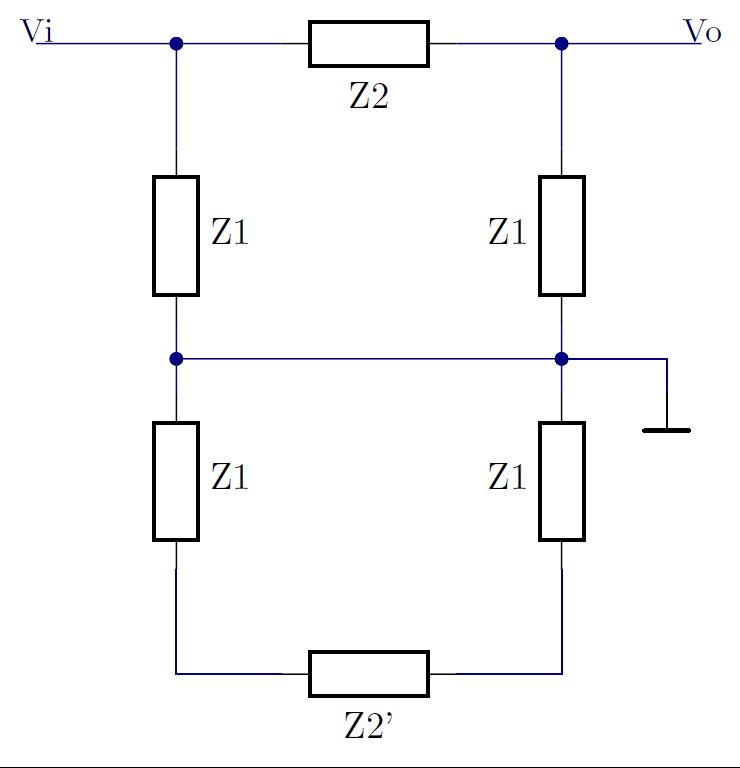
\includegraphics[width=0.4\textwidth, trim={0 0.1cm  0 0.1cm},clip]{ej1kennellly.jpg}
\caption{Filtro Twin T Notch luego de aplicar el teorema de Kenelly.}
	\label{fig:filtrosimplificado}
\end{figure}

Luego, se observa que el circuito puede simplificarse aún mas teniendo en cuenta las impedancias en paralelo. Finalmente, se obtiene el circuito mostrado en la Figura (\ref{fig:filtrofinal}).

\begin{figure}[H]
	\centering
	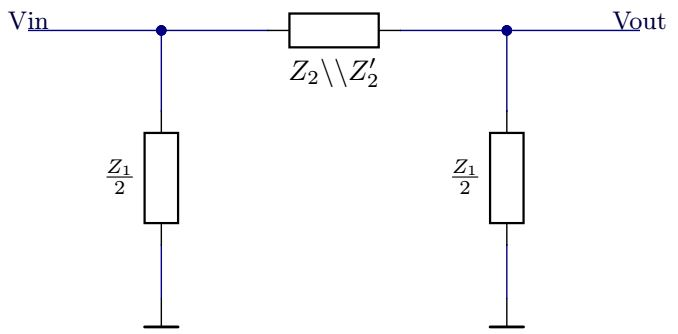
\includegraphics[width=0.6\textwidth]{ej1simplificado.jpg}
\caption{Filtro Twin T Notch simplificado.}
	\label{fig:filtrofinal}
\end{figure}

Realizando los cálculos de la transferencia en el circuito simplificado, se obtiene que
\[ \frac{Vo}{Vi}=H(S)=\left( \frac{SCR}{1+SCR} \right)^2 \] 
Luego, la respuesta en frecuencia será
\[H(j\omega)=\left( \frac{j 2\pi f CR}{1+ j2\pi f CR} \right)^2 \]
Antitransformando por Fourier, se obtiene la respuesta impulsiva
%\[h(t)=\frac{-2}{CR}e^{\frac{-t}{CR}}+\frac{t}{(CR)^2}e^{\frac{-t}{CR}}\]

\[h(t)=\left( -2 + \frac{t}{CR} \right)\frac{e^{\frac{-t}{CR}}}{CR} \]


\subsection{Ejercicio 2: Filtro pasa-bajos RC}
Se simuló y se armó en un protoboard un filtro pasa-bajos RC, seleccionando los valores de los componentes adecuados para lograr que la frecuencia de corte sea de $ 48 \ kHz $. Los componentes utilizados fueron dos resistencias, una de $22 \ \Omega$ y otra de $680 \ \Omega$ y un capacitor de $4.7 \ nF$, contemplando los valores comerciales.
Dicho circuito fue alimentado con una señal cuadrada de $ 10 \ V_{PP} $ con una frecuencia de $ 24 \ kHz $.
En forma teórica se llegó a ...
Por un lado, las simulaciones se muestran en la Figura (\ref{fig:simu2}).

\begin{figure}[H]
	\centering
	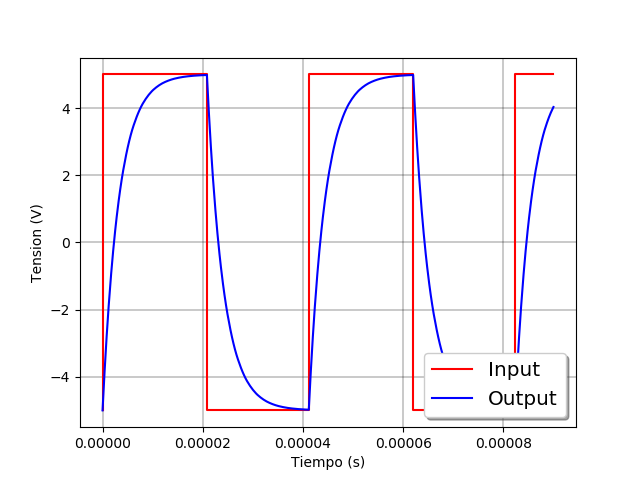
\includegraphics[width=0.9\textwidth]{Entrada-Salida.png}
\caption{Entrada (en azul) y salida (en amarillo) del circuito armado.}
	\label{fig:simu2}
\end{figure}

Por otro lado, las mediciones se observan en la Figura (\ref{fig:medicion2}). Cabe destacar que en dicha figura, la señal cuadrada de la fuente no posee una forma cuadra perfecta debido a la baja impedancia de entrada de la fuente.

\begin{figure}[H]
	\centering
	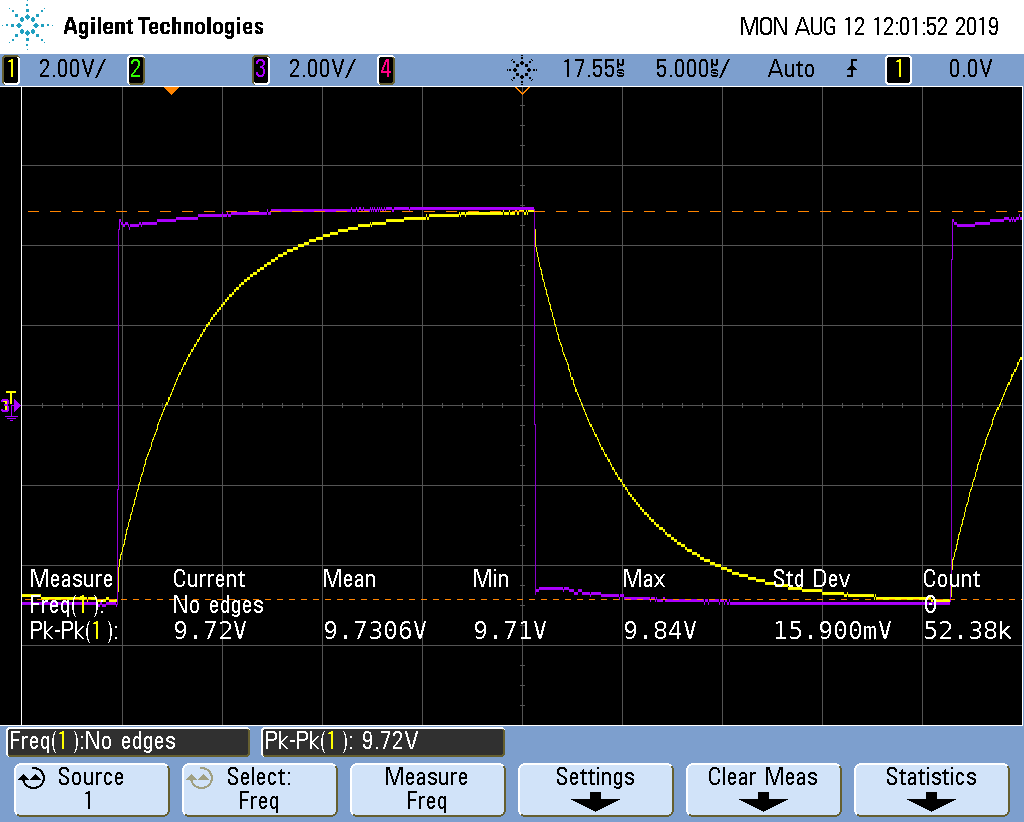
\includegraphics[width=0.9\textwidth , trim={0.7cm 6.25cm  0 3.5cm},clip]{scope_1}
	%trim={<left> <lower> <right> <upper>}
\caption{Entrada (en violeta) y salida (en amarillo) del circuito armado.}
	\label{fig:medicion2}
\end{figure}

Repitiendo las mediciones con una señal de las mismas características, pero con una frecuencia de $ 480 \ Hz $ se observó ...

Finalmente, se puede observar que dicho circuito puede ser utilizado como un integrador atenuado a muy altas frecuencias, ya qué

\begin{equation}
	H \left(S \right) = \frac{1}{SRC \ + 1} \approx \frac{1}{RC} \cdot \frac{1}{S}
\end{equation}

\subsection{Ejercicio 3: Plot Tool 2019}
Finalmente, en este punto se programó una GUI en Phyton que permite realizar gráficos de diagramas de BODE. Dicho programa permite analizar funciones transferencia analíticas, archivos de LTSpice, ... 
Ademas de comparar con facilidad varios diagramas de BODE y de diversas fuentes, el programa permite ...

\section{Conclusiones}


\end{document}
